% Appendix A: ten archive pictures with their human labels and the corrected design's three answers.

This appendix shows ten pictures from the archive with their human scene labels and the three answers the corrected design (Chapter~\ref{ch:corrected_design}) gives for them. Rater~A is the expert who reviewed the first $801$ pictures of the labelled pool; Rater~B is the author, who annotated the $300$ pictures of the spatial audit.
\begin{itemize}
    \item \textbf{Scene at all} (the first level): $p$ is the combined probability of a scene, with mappings fitted on the $749$ training pictures of the fixed split and the pool's labels as used for the main results; the call is ``scene'' when $p \ge 0.5$, and it is approved without a person when conformal risk control at $\alpha = 0.05$, calibrated on the split's $252$ calibration pictures, puts its uncertainty below the cut-off ($0.829$).
    \item \textbf{Scene class} (Section~\ref{sec:scene_classes}): the most probable of the six answers, with its probability, from the system's learned combination fitted under one definition of a scene on the same split; ``approved'' means the risk promise at $\alpha=0.05$ accepts the answer without a person. The short list is the set at $\alpha=0.10$.
    \item \textbf{Objects} (Section~\ref{sec:objects_llava_vs_fusion}): the list of object classes under a promise that at most $10\%$ of objects are missed, with mappings fitted on books of the $300$ hand-annotated pictures that contain none of these ten pictures.
\end{itemize}
Five of the six pictures with a pool label were among the pictures the design was fitted or calibrated on, so the examples illustrate the decisions; they are not evidence of accuracy, which Chapter~\ref{ch:corrected_design} measures on held-out books.

The pictures make two points of the main text visible. First, many pictures in the archive are ornaments, borders and small sketches rather than scenes. The expert labels count them as ``drawing'', and so as scenes, and the first level, fitted on those labels, calls all ten pictures scenes. Second, under one definition of a scene (Section~\ref{sec:archive_check}) the scene-class design calls the five ornaments ``no scene'' with confidence and approves them, while the figurative pictures receive a class; the specific scene classes are the hard part, as Section~\ref{sec:scene_classes} reports.

\begin{figure}[!htbp]
    \centering
    \begin{subfigure}[t]{0.48\textwidth}
        \centering
        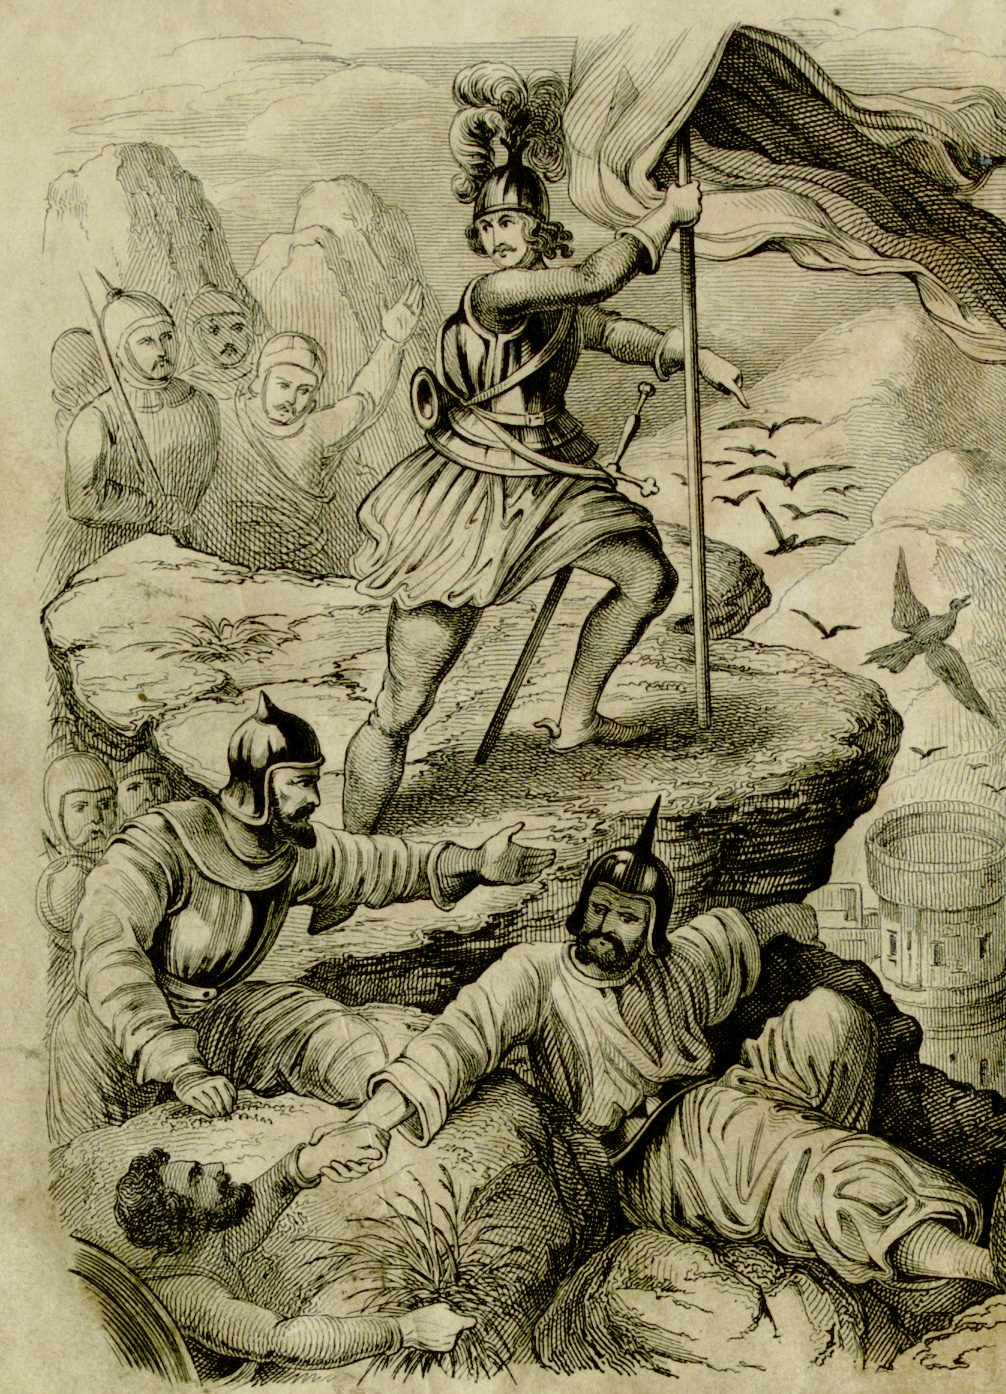
\includegraphics[width=\linewidth,height=4.6cm,keepaspectratio]{latex_assets/failure_degraded_2.jpg}
        \caption{\texttt{PPN1802793658/00000080\_0}. Soldiers with a banner on a rock. Labels: drawing (A), playing (B). Scene: $p = 0.980$, approved. Class: drawing ($0.947$), approved. Objects: person, animal, weapon.}
    \end{subfigure}
    \hfill
    \begin{subfigure}[t]{0.48\textwidth}
        \centering
        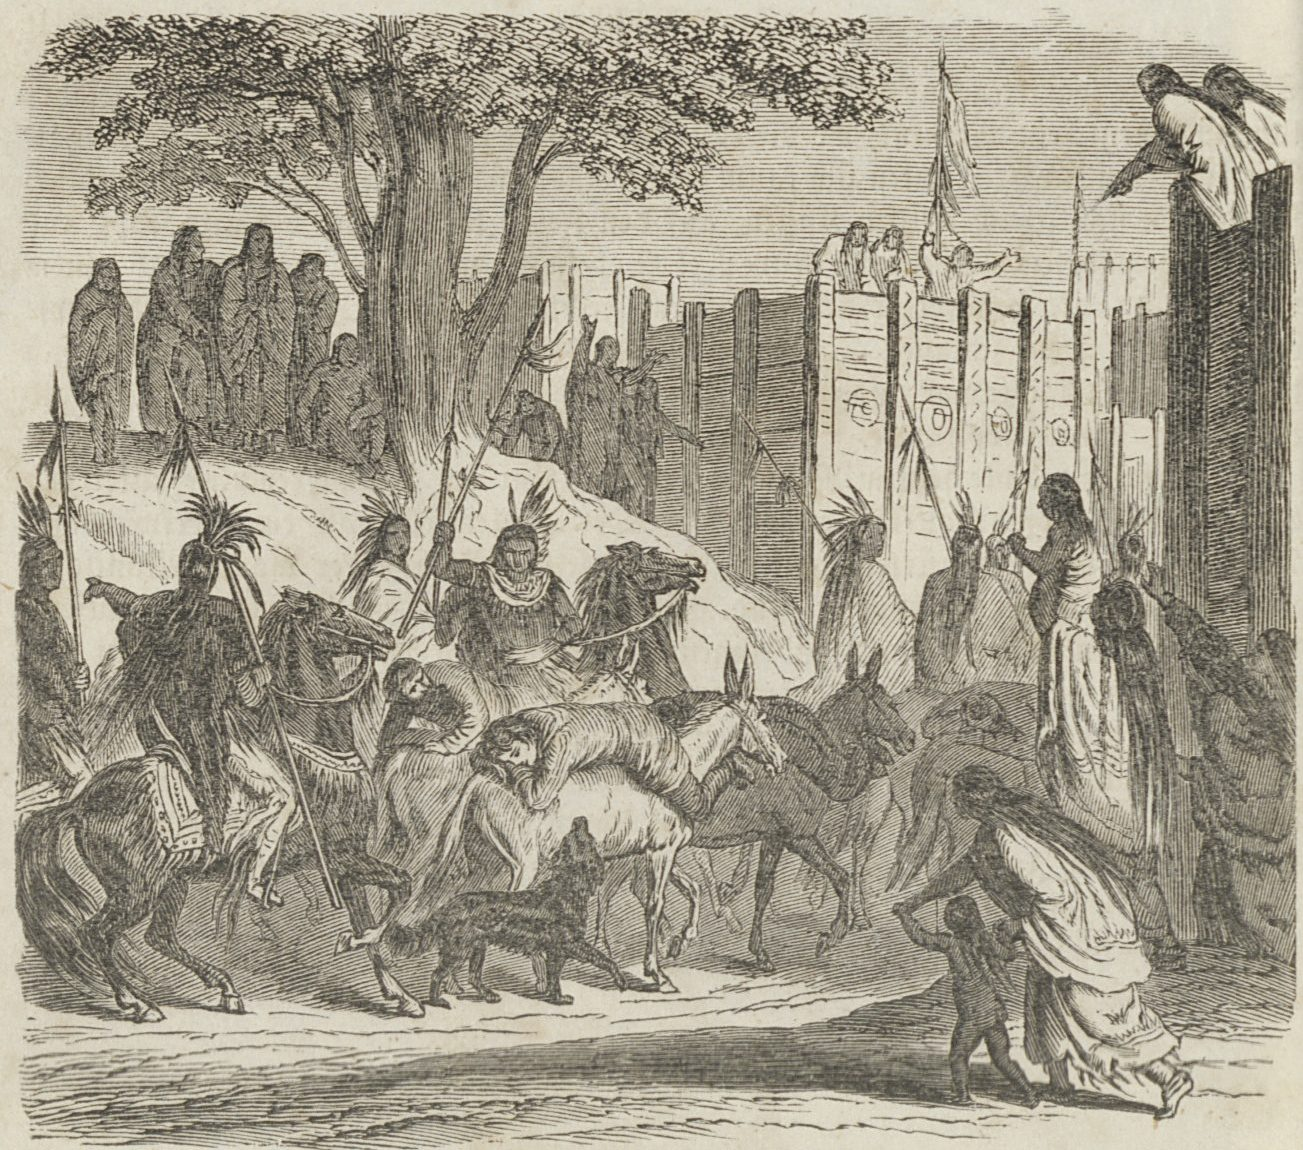
\includegraphics[width=\linewidth,height=4.6cm,keepaspectratio]{latex_assets/failure_crowded_2.jpg}
        \caption{\texttt{PPN1837132763/00000240\_0}. Riders, people and a dog before a palisade. Label: playing (B, $12$ boxes); not in the pool. Scene: $p = 0.993$, approved. Class: drawing ($0.807$), approved. Objects: person, child, animal, building, weapon, tree.}
    \end{subfigure}

    \vspace{3mm}

    \begin{subfigure}[t]{0.48\textwidth}
        \centering
        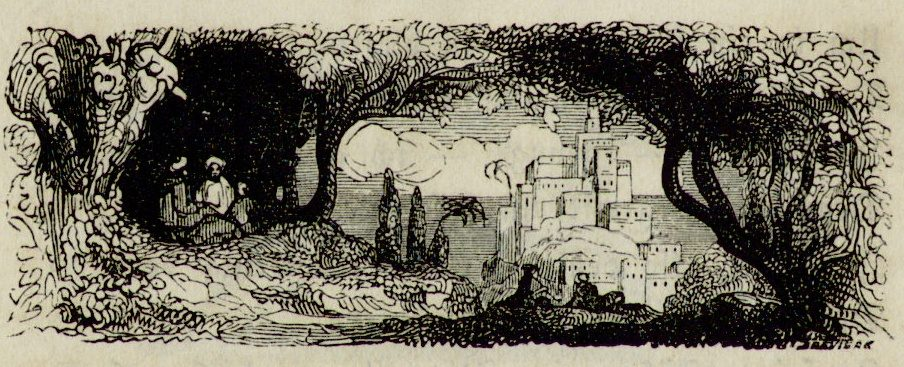
\includegraphics[width=\linewidth,height=4.6cm,keepaspectratio]{latex_assets/failure_drawing_1.jpg}
        \caption{\texttt{PPN1816431109/00000460\_0}. Trees, figures and a town by the sea. Labels: landscape (A), drawing (B); a test picture. Scene: $p = 0.920$, approved. Class: landscape ($0.582$), not approved; list landscape, drawing. Objects: person, building, tree.}
    \end{subfigure}
    \hfill
    \begin{subfigure}[t]{0.48\textwidth}
        \centering
        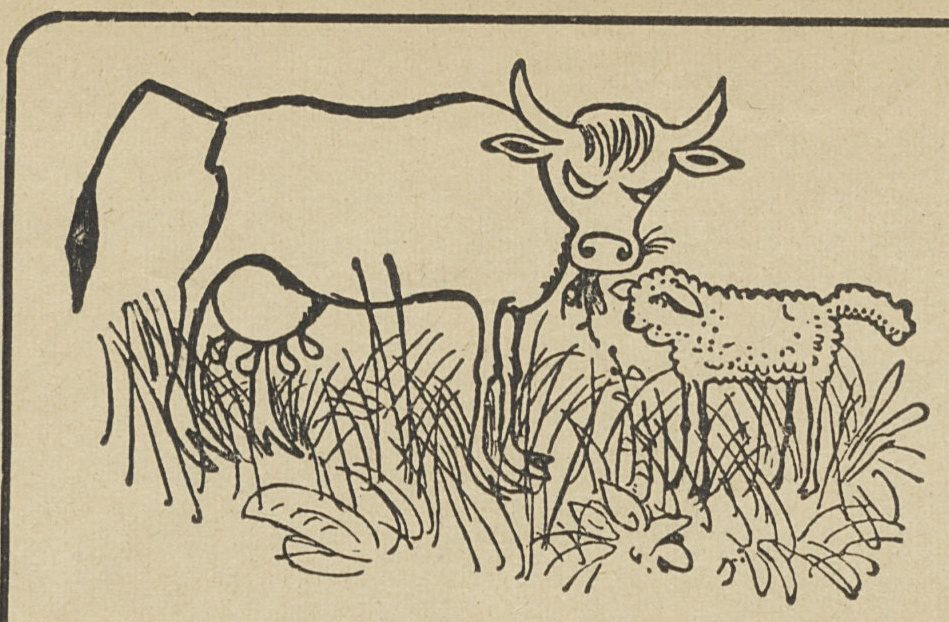
\includegraphics[width=\linewidth,height=4.6cm,keepaspectratio]{latex_assets/failure_occlusion_2.jpg}
        \caption{\texttt{PPN1859148263/00000091\_1}. A cow and a sheep in grass. No human label. Scene: $p = 0.922$, approved. Class: drawing ($0.516$), not approved; list drawing, no scene. Objects: animal.}
    \end{subfigure}
    \caption[Four scenes and the design's answers]{Four scenes. The first level approves all four as scenes. The scene classes are harder: the two raters give the first and third pictures different classes (drawing against playing, landscape against drawing), the disagreement Section~\ref{sec:cohort_taxonomy} measures; the design approves ``drawing'' for the first two, where Rater~B said playing for the second, and sends the other two to a person. For the third it names landscape first, Rater~A's class, with Rater~B's drawing second on its short list. The object lists name what is there, with an extra class or two to strike out.}
    \label{fig:example_scenes}
\end{figure}

\begin{figure}[!htbp]
    \centering
    \captionsetup[sub]{font=footnotesize}
    \begin{subfigure}[t]{0.31\textwidth}
        \centering
        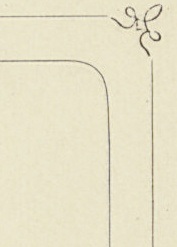
\includegraphics[width=\linewidth,height=3.6cm,keepaspectratio]{latex_assets/failure_degraded_1.jpg}
        \caption{\texttt{PPN183128149X/00000083\_1}. Corner of a frame. Label: no scene (B). Scene: $p = 0.639$, not approved. Class: no scene ($0.983$), approved. Objects: none.}
    \end{subfigure}
    \hfill
    \begin{subfigure}[t]{0.31\textwidth}
        \centering
        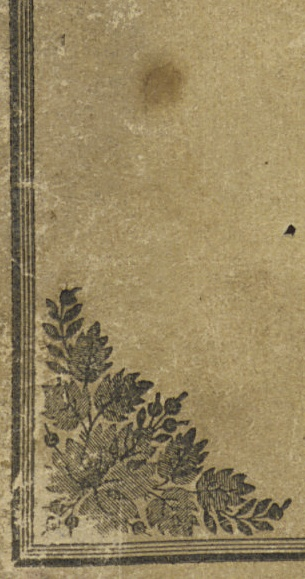
\includegraphics[width=\linewidth,height=3.6cm,keepaspectratio]{latex_assets/failure_drawing_2.jpg}
        \caption{\texttt{PPN1807545539/00000142\_0}. Leaf ornament in a page corner. Labels: drawing (A, B). Scene: $p = 0.624$, not approved. Class: no scene ($0.988$), approved. Objects: none.}
    \end{subfigure}
    \hfill
    \begin{subfigure}[t]{0.31\textwidth}
        \centering
        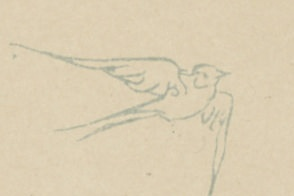
\includegraphics[width=\linewidth,height=3.6cm,keepaspectratio]{latex_assets/failure_occlusion_1.jpg}
        \caption{\texttt{PPN176263855X/00000017\_4}. Faint sketch of a swallow. Labels: drawing (A, B). Scene: $p = 0.933$, approved. Class: drawing ($0.564$), not approved; list drawing, no scene. Objects: person, animal.}
    \end{subfigure}

    \vspace{3mm}

    \begin{subfigure}[t]{0.31\textwidth}
        \centering
        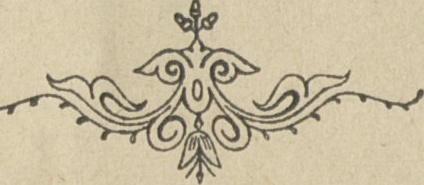
\includegraphics[width=\linewidth,height=3.6cm,keepaspectratio]{latex_assets/failure_crowded_1.jpg}
        \caption{\texttt{PPN175936214X/00000010\_0}. Decorative headpiece. Label: drawing (A). Scene: $p = 0.621$, not approved. Class: no scene ($0.985$), approved. Objects: none.}
    \end{subfigure}
    \hfill
    \begin{subfigure}[t]{0.31\textwidth}
        \centering
        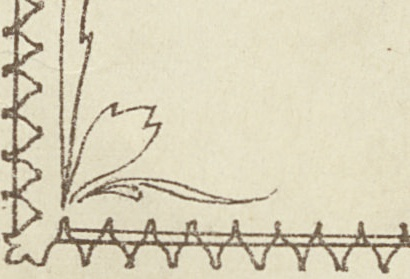
\includegraphics[width=\linewidth,height=3.6cm,keepaspectratio]{latex_assets/failure_text_conflict_1.jpg}
        \caption{\texttt{PPN1837925887/00000046\_0}. Corner of a border. No human label. Scene: $p = 0.623$, not approved. Class: no scene ($0.996$), approved. Objects: weapon.}
    \end{subfigure}
    \hfill
    \begin{subfigure}[t]{0.31\textwidth}
        \centering
        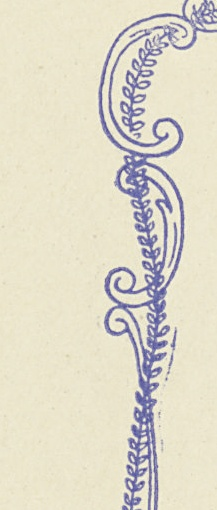
\includegraphics[width=\linewidth,height=3.6cm,keepaspectratio]{latex_assets/failure_text_conflict_2.jpg}
        \caption{\texttt{PPN1859200435/00000091\_1}. Scroll ornament. No human label. Scene: $p = 0.670$, not approved. Class: no scene ($0.967$), approved. Objects: none.}
    \end{subfigure}
    \caption[Six ornaments and sketches and the design's answers]{Six ornaments and sketches. The first level, fitted on labels that count ornaments as ``drawing'', calls all six scenes but approves only the sketch (c); the five ornaments go to a person, because it is unsure. Under one definition of a scene the scene-class design calls the five ornaments ``no scene'' with confidence and approves them, including those the expert labelled ``drawing'': the two definitions of Section~\ref{sec:scene_definition} lead to opposite answers on the same picture. The sketch of a swallow (c) is a drawing under both, and its object list adds a person that is not there.}
    \label{fig:example_ornaments}
\end{figure}
